\chapter{Marco Teórico} \label{chapter:chapter2}

\section{Aprendizaje automático}
El aprendizaje automático es un subcampo de la ciencias de la computación y una rama de la inteligencia artificial cuyo objetivo es resolver una tarea basándose en alguna experiencia, algunos ejemplos clarificadores de tareas a resolver pueden ser clasificar si un correo electrónico es spam o no, traducción automática de textos, reconocimiento de voz o reconocimiento facial. Cuando nos referimos a la experiencia estamos hablando generalmente del conjunto de datos que usaremos para poder entrenar los diferentes algoritmos para poder resolver dichas tareas. Los algoritmos que se utilizan en el aprendizaje automático pueden ser categorizados en el mayor de los casos como supervisados o no supervisados, la diferencia de ambos radica en el conjunto de datos con los cuales son entrenados, a continuación vamos a explayarnos y tratar de clarificar la diferencias de ambos.

\subsection{Aprendizaje supervisado}
En el aprendizaje automático supervisado al momento del entrenamiento contamos con un conjunto de datos en los cuales para cada ejemplo del mismo sabemos la predicción correcta, \textit{tag} o \textit{label}, dejando explícitamente la relación entre la entrada y salida del algoritmo. Generalmente las tareas que podemos resolver con este subconjunto de algoritmos pueden ser categorizados en problemas de regresión y clasificación, para los primeros se predicen valores continuos, lo cual significa que estamos tratando de relacionar las variables de entrada en una función continua, para los problemas de clasificación se predicen valores discretos, lo cual significa que tratamos de relacionar las variables de entrada en categorías bien definidas. Ejemplos bien concretos de ambos enfoques pueden ser predecir la edad de una persona dada una imagen de la misma, para una regresión, la edad es una variable continua y para una clasificación predecir si un correo electrónico es spam o no.

\subsection{Aprendizaje no supervisado}
El aprendizaje automático no supervisado difiere del supervisado en que no se dispone de la salida correcta a cada ejemplo de el conjunto de datos. Este tipo de algoritmos nos permiten aproximar problemas sin contar a priori con información de cómo están compuestos nuestros datos, un tipo claro de estos algoritmos es el agrupamiento, mayormente conocido como \textit{clustering} en inglés, un ejemplo de este tipo de problemas o tarea podría ser la segmentación por algún comportamiento en común de usuarios en la red social Twitter.


\subsection{Ejemplo: Predicción del valor de la vivienda}
Vamos abordar diferentes conceptos del aprendizaje automático tales como el modelo, la función de pérdida y el algoritmo de aprendizaje a través de un ejemplo concreto simplificado, este será la predicción del valor de una vivienda.
Para empezar vamos a describir el conjunto de entrenamiento, sea  $C = \{(x_{i}, y_{i})\}_{i=0}^{N}$ el dataset donde $N$ son la cantidad de datos que tenemos disponibles y para cada uno de estos tenemos $x_{i}$ que va a ser nuestra única variable de entrada que representa la cantidad de metros cuadrados de la vivienda e $y_{i}$ que representa el valor monetario de la misma. Con la descripción del problema antes mencionado podemos decir que se tratará de un algoritmo de aprendizaje automático supervisado, más aún es un problema de regresión ya que necesitamos predecir el valor de la vivienda y esto es continuo. Ya sabemos como son los datos ahora falta definir el modelo, o sea la función que vamos a proceder a entrenar, queremos tener una $f^{*} : \mathbb{R} &\mapsto \mathbb{R}$ (función de reales en reales) tal que tome como entrada el tamaño de la vivienda y retorne el costo de la misma. La forma más fácil de representarla es con una función lineal como puede ser $f(x; \theta) = x * \theta_{1} + \theta_{0} $ donde $\theta$ son los parámetros del modelo.
Ya tenemos bien definidos como son los datos y el modelo, ahora bien una pregunta que surge naturalmente sería ¿Como sabemos cuán bien está prediciendo el modelo? ¿Cómo podemos decidir qué valores de $\theta$ son mejores que otros?, para responder estas preguntas vamos a introducir la función de pérdida o costo, vale aclarar que para cada problemática vamos a utilizar alguna función de costo acorde a la misma, para la situación de nuestro ejemplo utilizaremos la función de error cuadrático medio la cual está definida de la siguiente manera 
$J(\theta_{0}, \theta_{1}) = \frac{1}{2N} * \sum_{i=0}^{N} (f(x_{i}; \theta_{0}, \theta_{1}) - y_{i})^{2}$ la cual nos dice cual es error del modelo dado ciertos parámetros fijos, nos resta definir cómo elegirlos de manera óptima para ello tendremos que minimizar $ \textit{argmin}_{\{\theta_{0}, \theta_{1}\}} J(\theta_{0}, \theta_{1}) $ ya que obtendremos los parámetros con el menor error posible. A continuación vamos a explayarnos en un algoritmo iterativo que se puede utilizar para este fin como lo es el descenso por el gradiente.

\subsection{Aprendizaje por descenso por el gradiente}
Sea $J : \mathbb{R}^{d} &\mapsto \mathbb{R}$ una función de costo y $ \theta \in \mathbb{R}^{d}$, tenemos como objetivo obtener los argumentos que minimicen el valor de salida de la funcion $J$, es decir, $ \textit{argmin}_{\theta} J(\theta) $. Para utilizar este algoritmo vamos a tener que hacer uso del gradiente $ \nabla J(\theta)$ que es el vector de derivadas parciales, donde $\frac{\zeta J(\theta)}{\zeta \theta_{i}}$ es la derivada parcial de $J$ con respecto a $\theta_{i}$.

El descenso por el gradiente es un algoritmo iterativo en el cual $\theta$ toma valores iniciales los cuales pueden ser aleatorios o fijos, y en cada iteración se actualizan simultáneamente los parámetros de la siguiente manera: $\theta_{j} := \theta_{j} - \alpha * \frac{\zeta J(\theta)}{\zeta \theta_{i}} $ donde $\alpha > 0 $ es el coeficiente o tasa de aprendizaje, conocido como \textit{learning rate}, el cual indica el tamaño del paso que damos en cada iteración del algoritmo, notar que con un $\alpha$ demasiado bajo se tardará mucho en converger a un mínimo, y con un learning rate demasiado alto el algoritmo puede llegar a diverger. En cada actualización de parámetros estamos dando un paso en dirección negativa del gradiente en determinado punto.

Ejemplo: supongamos que queremos minimizar $f(w) = w^{2}$, calculamos la derivada $f^{'}(w) = 2w$, determinemos un $\alpha = 0.1 $ y un valor inicial aleatorio de $w = -8$, en la primera iteración del algoritmo vamos a tener un valor de $w = w - f^{'}(w) = -6.4$ siguiendo la iteración del algoritmo vamos a llegar a un valor mínimo, en este ejemplo ese valor sería $w = 0$. En la Figura \ref{fig:decenso_por_el_gradiente} podemos ver cómo se va actualizando el valor de $w$ hasta converger.

\begin{figure}
\begin{center}
    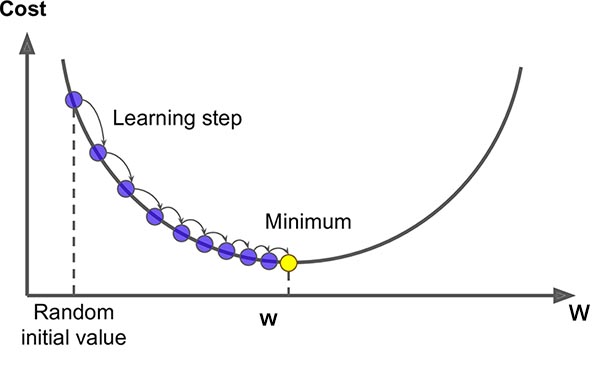
\includegraphics[width=\textwidth]{images/image206.png}
    \caption{Descenso por el gradiente de la funcion $f(w) = w^{2}$}
    \label{fig:decenso_por_el_gradiente}
\end{center}
\end{figure}


\section{Redes Neuronales}
Las redes neuronales son una composición de funciones no lineales donde el objetivo principal es tratar de estimar de nuevo los parámetros $W$ de $f(X; W,b)$ donde esta $f$ está definida como $f_{n} \circ ... \circ f_{0}(X)$, la particularidad de que sean funciones no lineales es poder representar estructuras más complejas, de hecho en el supuesto de que todas las $f_{i}$ sean lineales la composición mencionada anteriormente sería otra función lineal, por lo tanto no tendría mucho sentido componerlas.
Cada $f_{i}$ se denomina como capa de la red neuronal, y está compuesta por perceptrones, la unidad básica de procesamiento.

\subsection{Perceptrón}
Como mencionamos/definimos anteriormente un perceptrón también conocido como neurona es la unidad básica de procesamiento que consta de múltiples entradas y una única salidas, las operaciones están dadas por las siguientes ecuaciones:

\[z = \frac{1}{n} * \sum_{i=1}^{n} x_{i}*w_{i} + b\]

\[y = f(z)\]

Donde $x_{1},..,x_{n}$ son los valores de entrada, $w_{1},..,w_{n}$ son los parámetros o pesos del modelo, y $f$ es la función de activación, en la siguiente sección veremos algunas posibles funciones. En la Figura \ref{fig:perceptron} vemos una representación de una neurona.

\begin{figure}
\begin{center}
    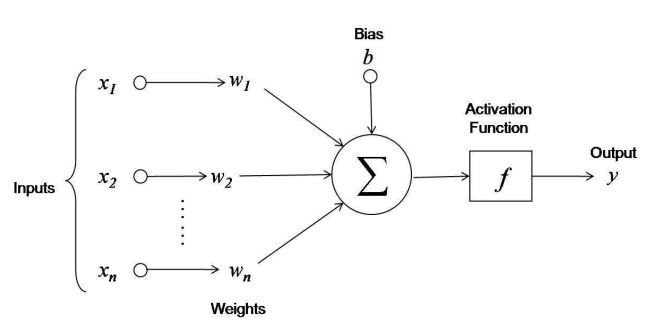
\includegraphics[width=\textwidth]{images/image204.png}
    \caption{Perceptrón}
    \label{fig:perceptron}
\end{center}
\end{figure}


\subsection{Redes Feedforward}
Estas redes neuronales se construyen uniendo y componiendo perceptrones en capas fully connected (completamente conectadas), un ejemplo de una red feedforward la podemos encontrar en la Figura \ref{fig:feedforward} , intuitivamente podemos decir que cada capa realiza una transformación no lineal del espacio vectorial de entrada en otro de salida.

\begin{figure}
\begin{center}
    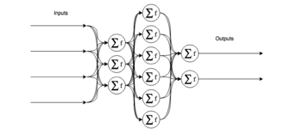
\includegraphics[width=\textwidth]{images/image210.png}
    \caption{Redes FeedForward}
    \label{fig:feedforward}
\end{center}
\end{figure}

El término de feedforward viene de que solo miran hacia adelante, la información fluye desde la entrada hacia la salida sin mirar hacia atrás, podemos representar el modelo como un grafo acíclico. Para poder entrenar estas redes normalmente se utiliza el algoritmo de backpropagation \cite{kelley1960gradient}.

\subsection{Activation}
Como vimos anteriormente en la Figura \ref{fig:perceptron} donde se explica el comportamiento del perceptrón se utiliza una función de activación, donde no la definimos. Dependiendo la problemática que deseamos atacar se utilizan diferentes funciones de activacion, en esta sección vamos a detallar las más conocidas.

Sigmoide:  \[ \sigma(x) = \frac{1}{1 + e^{-x}}\]

Es una función continua no lineal donde toma cualquier rango de los números reales y el valor de salida está comprendido entre $0$ y $1$. En la Figura \ref{fig:sigmoid} podemos ver la gráfica de la misma.

\begin{figure}
\begin{center}
    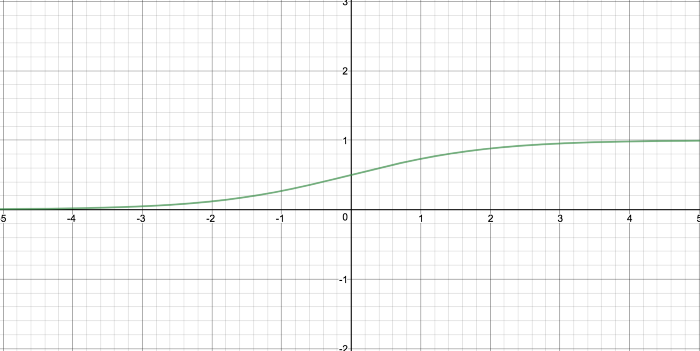
\includegraphics[width=\textwidth]{images/image216.png}
    \caption{Sigmoide}
    \label{fig:sigmoid}
\end{center}
\end{figure}

ReLU:  \[ReLU(x) = max(0, x)\]

ReLU, \textit{rectified linear unit}, por sus siglas en inglés, es una función muy simple que dado un valor, si es negativo devuelve $0$, caso contrario el mismo valor. En la Figura \ref{fig:relu} se detalla la grŕafica.

\begin{figure}
\begin{center}
    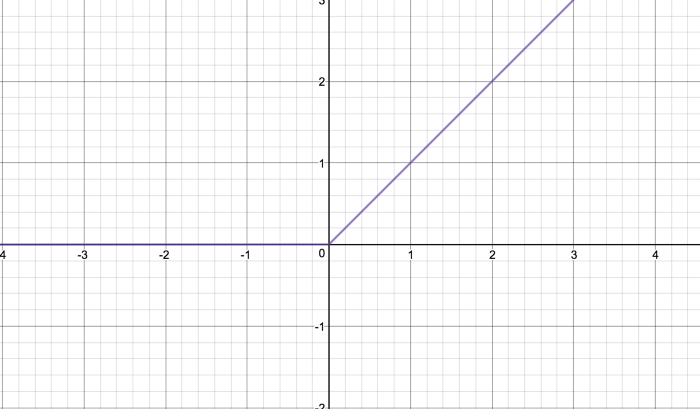
\includegraphics[width=\textwidth]{images/image213.png}
    \caption{ReLU}
    \label{fig:relu}
\end{center}
\end{figure}

\section{Redes Neuronales Convolucionales}

Las Redes Neuronales Convolucionales (\textit{CNNs}, del ingles, Convolutional Neural Networks) son una expresión de las Redes Neuronales especializadas en procesar datos de naturaleza de grilla como lo son los datos de series temporales, pueden verse como una grilla \textit{1-D}, y las imágenes que se puede pensar como una grilla \textit{2-D}. El nombre se debe a que se utiliza una operación matemática llamada convolución. Se llaman \textit{CNNs} a una \textit{NN} que utiliza una convolución en vez de una multiplicación matricial en al menos una capa. En esta sección vamos a explicar la convolución y sus ventajas, el pooling y por último vamos ver una arquitectura de CNN como lo es la \textit{VGG} que es la que se utilizará a lo largo del trabajo.

\subsection{Convolución}

La convolución se denota como $s(t) = (x * w) (t)$, donde $x$ y $w$ son funciones, en el dominio de las imágenes puede pensarse que $x$ se refiere al input, $w$ al \textit{kernel}, y la resultante sería el \textit{feature map}, en el aprendizaje automático el input puede pensarse como un \textit{tensor} de datos y el kernel como uno de parámetros, la convolución en su forma discreta se define como $s(t) = (x * w) (t) = \sum_{a=-\infty}^{a=\infty} x(a) w(t - a)$. En la Figura \ref{fig:convolution} podemos ver un ejemplo de una convolución \textit{2-D} cuya particularización de la definición es $s(i, j) = (I * K) (i, j) = \sum_{n}^{m} I(i+m, j+n) K(m, n)$. Notar que el kernel recorre el input de a saltos de $1$ fila/columna, $stride = 1$, de la grilla y que la dimensionalidad del output es menor que la del input, estas condiciones se pueden modificar adrede de acuerdo al caso de uso que se necesite, por ejemplo podemos mantener la dimensionalidad haciendo uso del \textit{padding} que consta de agregar una fila y columna al input, existen diferentes tipos de padding que no se verán en el presente trabajo.

\begin{figure}
\begin{center}
    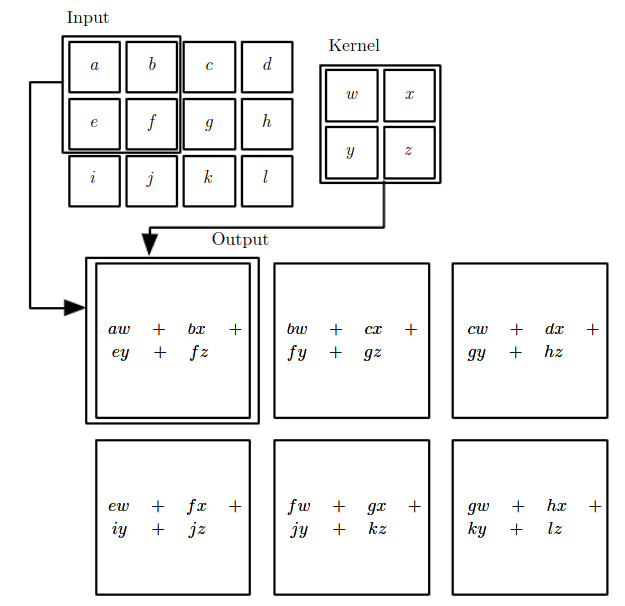
\includegraphics[width=\textwidth]{images/image200.png}
    \caption{Convolución}
    \label{fig:convolution}
\end{center}
\end{figure}

Utilizar convoluciones en vez de capas densas nos da ventajas como lo son las conecciones esparsas y la noción de pesos compartidos, esto se debe a que en las capas dense por cada output tenemos interacciones con cada input, en cambio con la convolución no, otra ventaja es que es menos costoso en memoria ya que posee menos parámetros y también en cálculo ya que se requieren menos operaciones.

\subsection{Pooling}

La capa de agrupación, \textit{pooling} en inglés, consiste en reducir la dimensionalidad del output de la capa anterior como lo puede ser en este contexto la convolución, existen diferentes tipos de pooling el más conocido es el max pooling, que consta de quedarse con el valor máximo, podemos ver un ejemplo en la Figura \ref{fig:pooling}. La intuición por detrás de este tipo de capas más allá del ahorro en cantidad de parámetros que se necesitarán aprender en las capas venideras es hacer invariante la arquitectura de CNNs a pequeñas traslaciones. Notar que no se aprenden parámetros en el pooling.


\begin{figure}
\begin{center}
    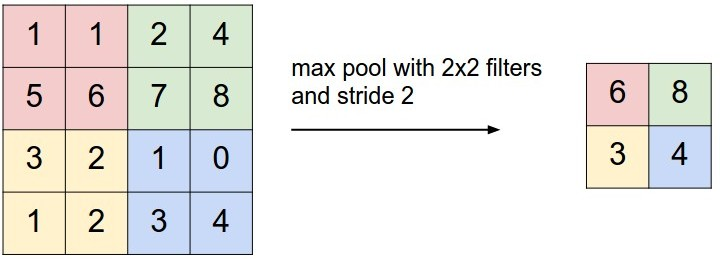
\includegraphics[width=\textwidth]{images/image220.jpg}
    \caption{Pooling}
    \label{fig:pooling}
\end{center}
\end{figure}

\subsection{VGG}

VGG \cite{VGG} es una familia de arquitecturas CNNs entrenadas para ImageNet \cite{imagenet_cvpr09} con el objetivo de poder clasificar una imagen entre las $1000$ categorías del \textit{dataset}. En la Figura \ref{fig:vgg19} podemos ver la arquitectura para una de ellas como lo es la \textit{VGG19}, podemos notar que está compuesta por bloques convolucionales, bloques densos y por último una softmax que nos da la distribución de probabilidad sobre las $1000$ categorías, en general cada bloque de una \textit{CNN} está compuesta por una capa de convolución seguida de una función no lineal y por último una capa de pooling, para el caso particular de la \textit{VGG19} cada bloque está compuesto por varias capas de Convoluciones de $3x3$ + \textit{ReLU}  seguido de un \textit{Max pooling}, y al final de los bloques de convoluciones podemos ver que tenemos dos capas densas, en la Figura \ref{fig:vgg19} se denota como \textit{FC1} y \textit{FC2}.

\begin{figure}
\begin{center}
    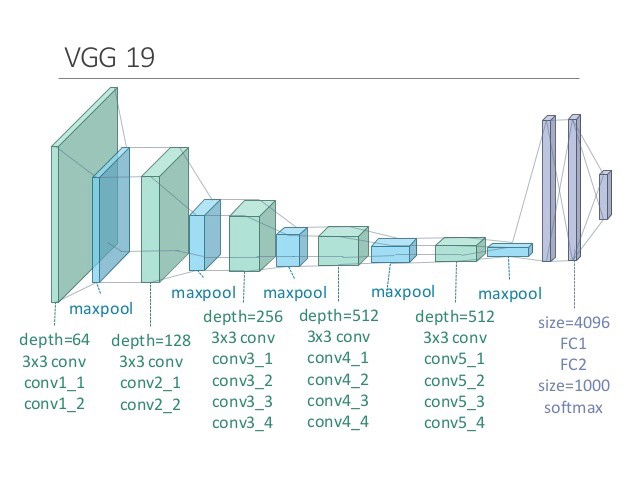
\includegraphics[width=\textwidth]{images/image197.jpg}
    \caption{VGG19}
    \label{fig:vgg19}
\end{center}
\end{figure}

En este trabajo se utilizará esta arquitectura para la extracción de features visuales, ¿Ahora bien cómo podemos realizar esto?, hay una noción en imágenes de que una \textit{CNN} entrenada en \textit{imageNet} generaliza bastante a otros dominio que no sea el de la competencia misma ya que se supone que \textit{ImageNet} son imágenes bastantes generales que han sido insertadas en la taxonomía de WordNet \cite{worNet}, ahora nuestro objetivo es extraer un vector que represente a una imagen, para hacer esto vamos a recortar/tirar la capa de clasificación de la \textit{VGG19} por lo tanto ahora cada vez que le demos como input una imagen vamos a obtener un vector de dimensionalidad $4096$.

\section{Word embeddings}

Una de las tareas más importantes dentro de PLN, procesamiento del lenguaje natural, es como representamos las palabras, teniendo como objetivo que estas sean el input, entrada, para cualquier modelo. Una característica fundamental en cómo representamos estas palabras es la noción de similitud entre las mismas por ejemplo la palabra “perro” tiene que tener una mayor similitud a “animal” que a la palabra “persona”, para poder atacar esta problemática vamos a hacer uso de vectores, por lo tanto cada palabra va a tener un vector en un espacio $N$ dimensional asociado que la representa, ahora bien la siguiente pregunta resultante fuera ¿Cómo generamos estos vectores?, el método más simple que podemos utilizar con ese objetivo es \textbf{one-hot vector} donde cada palabra $w \in \mathbb{R}^{|V|}$ siendo $V$ el vocabulario ordenado, $w$ consiste en todos ceros y un único uno en el índice que representa la palabra en $V$, a continuación daremos un ejemplo para clarificar cómo funciona este método: supongamos que tenemos la sentencia \textit{el perro ladra} por lo tanto $V$ = [\textit{el}, \textit{ladra}, \textit{perro}] , $|V| = 3$,  por lo tanto los vectores de palabras serían los siguientes: $"el" = [1, 0, 0]$, $"ladra" = [0, 1, 0]$, $"perro" = [0, 0, 1]$. Ahora con esta representación vectorial al ser cada palabra una entidad completamente independiente no captura una propiedad que si nos importaba como lo es la similitud entre las palabras.
A continuación vamos a ver cómo podemos capturar esta noción mediante dos algoritmos como lo son \textbf{word2vec} \cite{mikolov2013efficient} y \textbf{Bert} \cite{devlin2018bert}.

\subsection{word2vec}

La idea detrás de este algoritmo es diseñar un modelo cuyo parámetros sean los word embeddings, vectores de palabras, luego entrenarlo con cierta tarea, y como nos explayamos anteriormente a cada iteración del entrenamiento, evaluamos el error y actualizamos los parámetros. Para poder generar estos embedding existen dos tipos de algoritmos, \textbf{CBOW} y \textbf{skip-gram} cada uno con diferentes objetivos.

\textit{CBOW} (Continuous bag of words): tiene como objetivo predecir la palabra central dentro de un contexto ($C$), palabras colindantes, por ejemplo en la sentencia \textit{el perro ladra} y un $C = 2$ vamos a tratar de predecir \textit{perro} dado [\textit{el}, \textit{ladra}]. En la Figura \ref{fig:word2vec_cbow} podemos ver el modelo \textit{cbow}, donde $C$ es el tamaño del contexto, $V$ es la longitud del vocabulario, $N$ es la dimensión de los word embeddings y $W, W'$ son los parámetros del modelo. En Algoritmo \ref{algo:cbow} podemos ver el procedimiento.

\begin{figure}
\begin{center}
    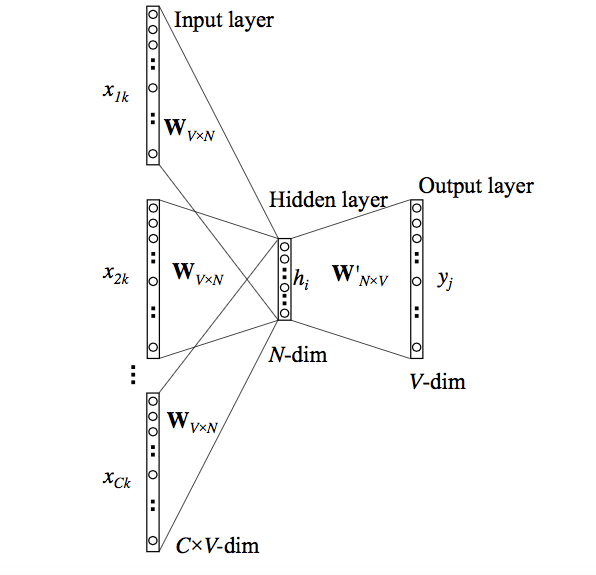
\includegraphics[width=\textwidth]{images/image219.png}
    \caption{CBOW}
    \label{fig:word2vec_cbow}
\end{center}
\end{figure}


\begin{algorithm}
\caption{CBOW}
\begin{algorithmic}[1]
\label{algo:cbow}
\STATE Generar los \textbf{one-hot vector} con las palabras del contexto, sean $x_{1}, \cdots , x_{C}$ estos vectores donde $x_{i} \in \mathbb{R}^{|V|}$. También para la palabra objetivo $y \in \mathbb{R}^{|V|}$.
\STATE Generar el word embedding promedio $h = \frac{v_{1} + \cdots + v_{C}}{C}$.
\STATE Generar el score vector $z = h \bullet W'$ donde $z \in \mathbb{R}^{|V|}$.
\STATE Transformar el score vector en probabilidades $\hat{y} = softmax(z) \in \mathbb{R}^{|V|}$.
\STATE Computar el error de la función objetivo cross entropy $H(y, \hat{y})$, actualizar los parámetros. Donde $H(y, \hat{y}) = −y log(\hat{y})$ y $softmax(z) = \frac{e^{z_{i}}}{\sum_{k = 1}^{|V|} e^{z_{k}}}$
\end{algorithmic}
\end{algorithm}

\textit{Skip-gram}: tiene como objetivo predecir las palabras de contexto a partir de la palabra central, por ejemplo para la sentencia antes mencionada \textit{el perro ladra} y un $C = 2$ vamos a tratar de predecir [\textit{el}, \textit{ladra}] dado \textit{perro}. En la Figura \ref{fig:word2vec_skip_gram} podemos ver el modelo \textbf{skip-gram}, donde $C$ es el tamaño del contexto, $V$ es la longitud del vocabulario, $N$ es la dimensión de los word embeddings y $W$, $W'$ son los parámetros del modelo. En Algoritmo \ref{algo:skip_gram} podemos ver el procedimiento detallado. Existe una optimización al momento del entrenamiento para el modelo skip-gram y este se basa en muestreo negativo \cite{MikolovSCCD13}

\begin{figure}
\begin{center}
    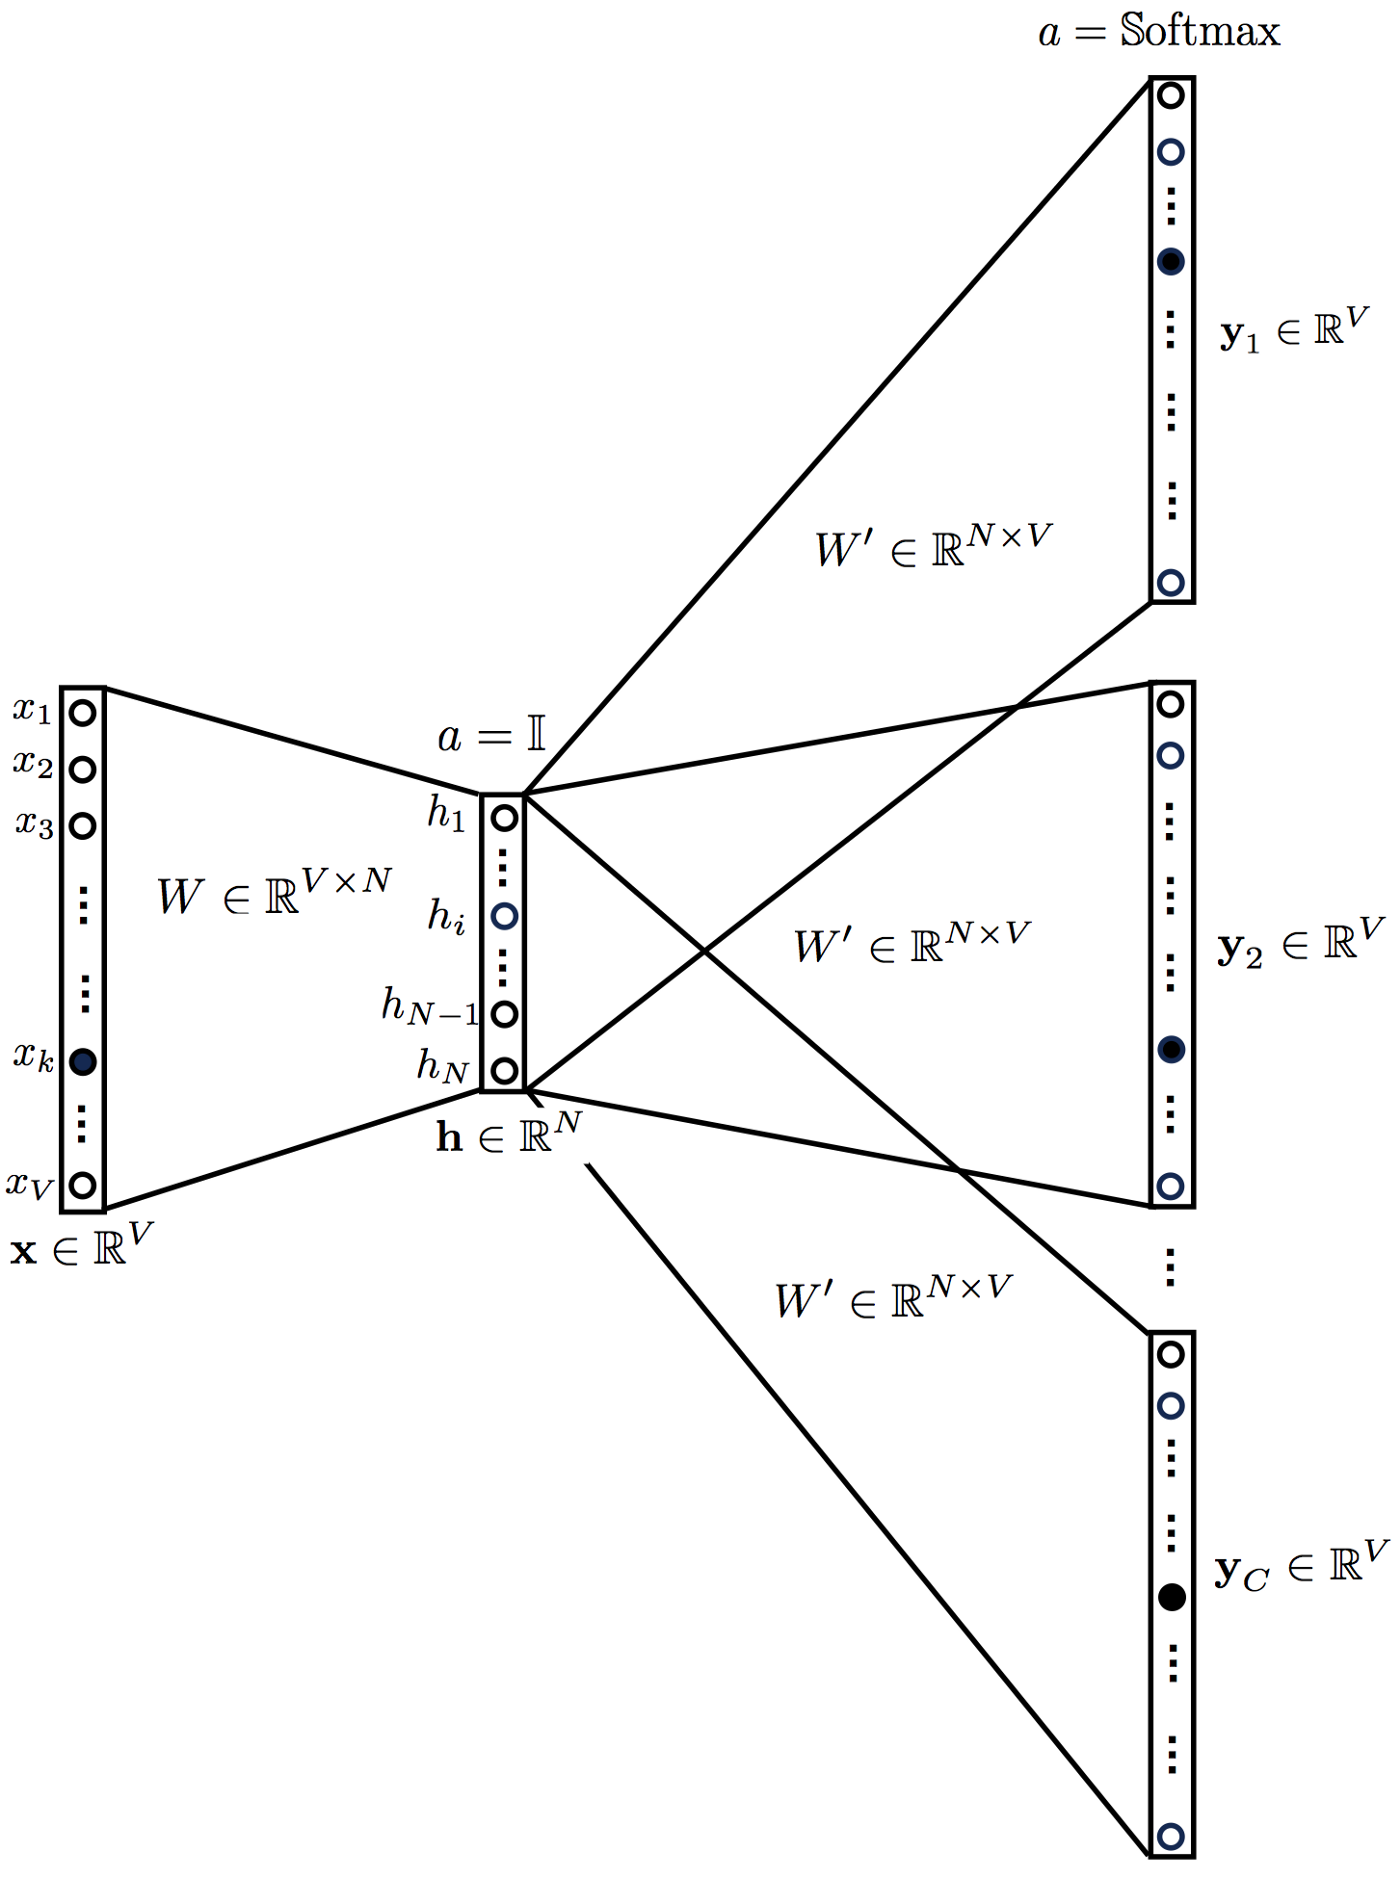
\includegraphics[width=\textwidth]{images/image211.png}
    \caption{SKIP-GRAM}
    \label{fig:word2vec_skip_gram}
\end{center}
\end{figure}


\begin{algorithm}
\caption{Skip-Gram}
\begin{algorithmic}[1]
\label{algo:skip_gram}
\STATE Generar los \textbf{one-hot vector} para la palabra central $x \in \mathbb{R}^{|V|}$ como también para las palabras del contexto que en este caso van a ser las objetivo $y_{1}, \cdots , y_{C} \in \mathbb{R}^{|V|}$.
\STATE Generar el word embeddings a partir de la palabra central, $v = x \bullet W$ donde $v \in \mathbb{R}^{N}$.
\STATE Generar el score vector $z = v \bullet W'$ donde $z \in \mathbb{R}^{|V|}$
\STATE Transformar el score vector en probabilidades $\hat{y} = softmax(z) \in \mathbb{R}^{|V|}$
\STATE Computar el error de la función objetivo cross entropy $H'(\hat{y}, y_{1}, \cdots , y_{C})$, actualizar los parámetros, donde $H'(\hat{y}, y_{1}, \cdots , y_{C}) = \sum_{i = 1}^{C} H (y, y_{i})$
\end{algorithmic}
\end{algorithm}

Notar que el hiper parámetro más importante en ambos modelos es $C$,la longitud del contexto. También tenemos que notar que una vez entrenado el modelo ya sea \textit{cbow} o \textit{skip-gram} nos quedamos con la matriz de parámetros $W’$ y $W$ respectivamente, estas van a ser los word embedding finales que se utilizaran con cierto propósito.

\subsection{Bert} \label{sec:bert}

Ciertos lenguajes de modelos pre entrenados han sido efectivos para mejorar algunas tareas de PLN, uno de ellos es Bert \cite{devlin2018bert}, Bidirectional Encoder Representation from Transformer, en esta sección veremos la arquitectura del modelo, como representar la entrada del mismo, como ha sido el proceso de entrenamiento y por último lo que realmente nos importa en este trabajo que es como generar embeddings a partir de este modelo pre entrenado.

\subsubsection{Arquitectura}

Es básicamente una pila de encoders del transformer, implementado y descrito en \cite{DBLP:journals/corr/VaswaniSPUJGKP17} , como podemos observar en la Figura \ref{fig:bert_arch} existe dos modelos diferentes. \textit{BERTbase} con una pila de $12$ encoder, $768$ hidden layer y $12$ self-attention heads $L=12$, $H=768$, $A=12$, $parámetros = 340M$. \textit{BERTlarge}, el cual contiene $L=24$, $H=1024$, $A=16$, $parámetros=110M$.

\begin{figure}
\begin{center}
    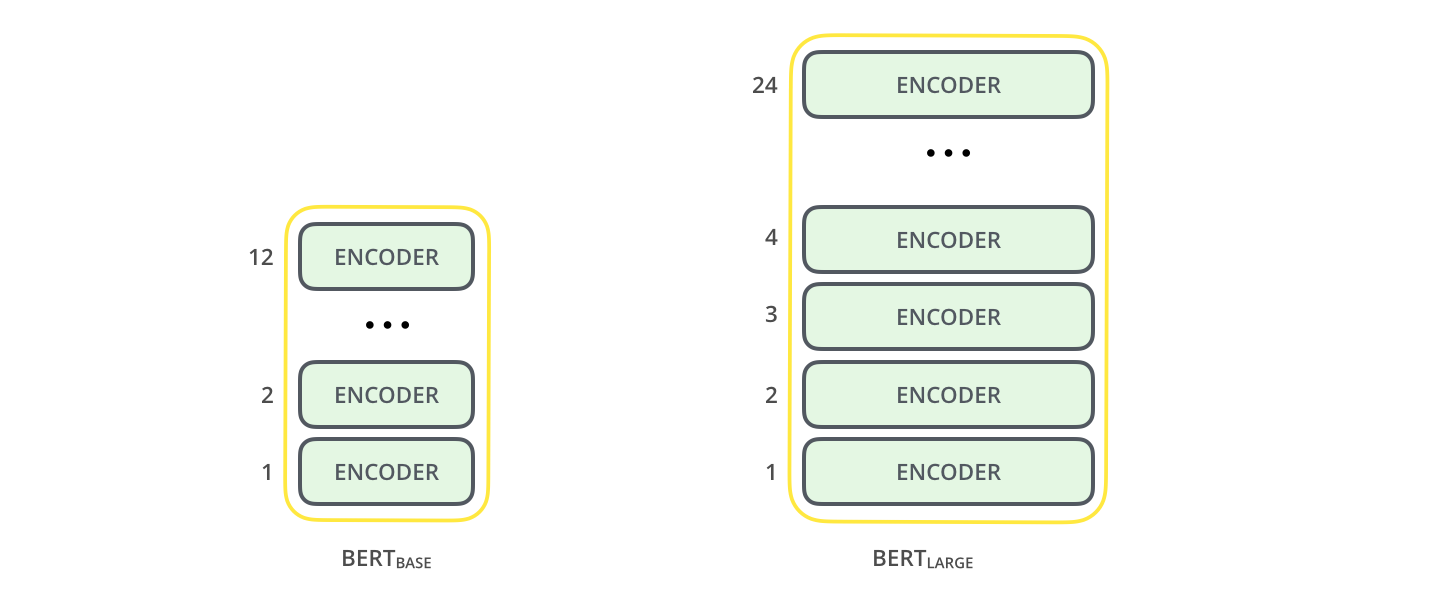
\includegraphics[width=\textwidth]{images/image209.png}
    \caption{Arquitectura de Bert \footnote{\url{http://jalammar.github.io/illustrated-bert/}}}
    \label{fig:bert_arch}
\end{center}
\end{figure}

Ahora que tenemos una noción del modelo vamos a mostrar cómo es un encoder del mismo. Nos enfoquemos en la Figura \ref{fig:encoder_arch} que nos muestra el funcionamiento del encoder para el caso de dos embeddings de entrada, lo primero a notar es que la información fluye hacia adelante en cada bloque del encoder, la primera capa es \textit{bidirectional self-Attention} en la cual no vamos a ondar, para ver su comportamiento se deja una lectura recomendada \textit{Attention is all you need} \cite{DBLP:journals/corr/VaswaniSPUJGKP17}, otra capa que tenemos es \textit{FFNN}, redes neuronales feedforward, con $4H$ de capas ocultas cada una, estas ya las describimos anteriormente, por último nos queda explicar que después de cada self-attention o feedforward tenemos una capa de normalización \cite{ba2016layer} la cual consta de conexiones residuales que lo único que hace es sumar la entrada y salida de la capa en cuestión y retorna esa suma hacia la siguiente capa.


\begin{figure}
\begin{center}
    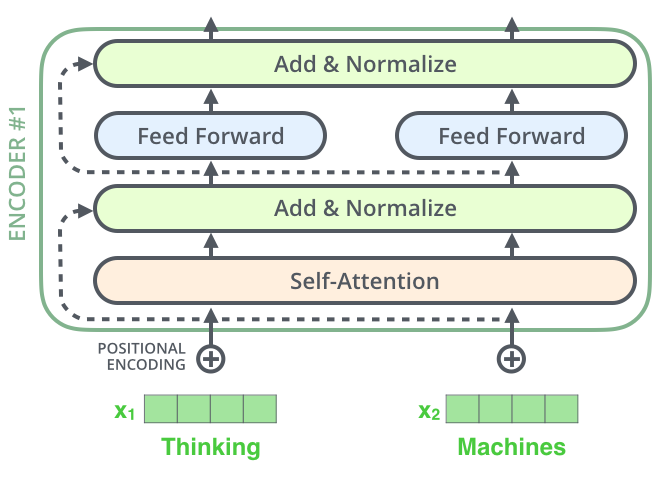
\includegraphics[width=\textwidth]{images/image217.png}
    \caption{Encoder \footnote{\url{https://jalammar.github.io/illustrated-transformer/}}}
    \label{fig:encoder_arch}
\end{center}
\end{figure}


\subsubsection{Representación de la entrada}

Una particularidad de \textit{BERT} es que puede tomar como entrada una o dos sentencias, por ejemplo para la tarea de Pregunta-Respuesta se utilizaría el segundo modelado de la entrada. Como factor común a todas las tareas que se quieran entrenar y/o hacer algún fine-tuning cada sentencia va a tener un token especial al principio como lo es \textit{[CLS]} y cada token es alineado con el algoritmo de \textit{WordPiece} \cite{45610}, para el caso de un modelo que requiera dos sentencias cada una de ellas va a estar separado por el token \textit{[SEP]}. Ahora a partir de estos token tenemos que generar un embedding para que sea la entrada al modelo, este embedding está compuesto por la sumatoria de tres diferentes embeddings, el primero es el token propiamente dicho, el segundo es un embedding que representa que sentencia es primera o segunda, y por último un embedding posicional del token con respecto a la sentencia. En la Figura \ref{fig:bert_input} podemos ver un ejemplo de esta representación.

\begin{figure}
\begin{center}
    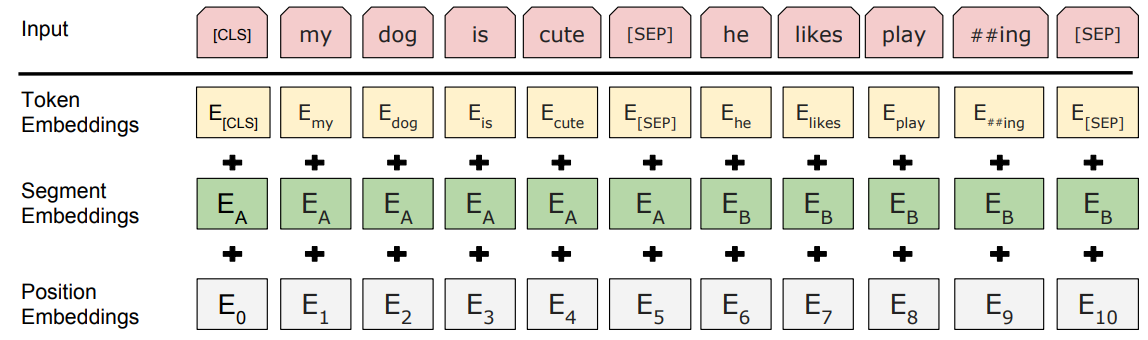
\includegraphics[width=\textwidth]{images/image201.png}
    \caption{Entrada de Bert}
    \label{fig:bert_input}
\end{center}
\end{figure}

\subsubsection{Entrenamiento}

Lo novedoso de \textit{BERT} es la forma que se entrenó el modelo de lenguaje, a diferencia de los modelos tradicionales donde se utiliza la técnica izquierda-derecha o viceversa, el pre-entrenamiento se basó en dos modelos no supervisados como \textit{MaskedLM} y \textit{predicción de la próxima sentencia}, en esta sección se datallará \textit{MLM}.
Los modelos clásicos no utilizaban modelos de lenguajes bidireccional ya que si queremos predecir algún token este indirectamente se puede estar viendo a si mismo, para atacar esta deficiencia el enfoque utilizado por \textit{BERT} fue ocultar, mask en inglés, un porcentaje de tokens de la sentencia de entrada de manera aleatoria y setearlos con el token especial \textit{[MASK]}, de esta manera la tarea sería predecir aquellos token \textit{[MASK]}, específicamente ese porcentaje fue $15\%$, a partir de esto surgen otros problemas a futuro, como por ejemplo ¿Como hacemos en un hipotético caso de fine-tuning?, esta discrepancia entre el pre entrenamiento y el fine-tuning se debe a que no se tiene el token \textit{[MASK]} en el último de estos, para abordar esta problemática se consideró que de ese $15\%$ de tokens que se reemplazan con el token especial, el $80\%$ se siguiera reemplazando de esa forma, otro $10\%$ que se reemplacen con algún token aleatorio, y el $10\%$ restante que se mantuviera el mismo token.

\subsubsection{Bert Embeddings} \label{sec:bert_emb}

Podemos usar el modelo pre entrenado para generar word embeddings contextualizados, lo podemos hacer de diferentes maneras ya que podemos tener un word embedding por capa de la arquitectura del modelo, por ejemplo en la Figura \ref{fig:bert_embeddings} si le damos como entrada al modelo la sentencia \textit{[CLS] el perro ladra} podemos extraer la salida de cada encoder y asociar el primer vector para el token \textit{[CLS]}, el segundo para \textit{perro} y el tercero para \textit{ladra}. En el paper \cite{devlin2018bert} los autores comparan diferentes formas de extracción de features para una tarea determinada en \textit{PLN} como lo es \textit{NER}, name entity recognition, y para ello utilizaron diferentes combinaciones que está bueno explayarse como tomar la primera capa del modelo (Embeddings de entrada), la salida del modelo, la ante última capa, la suma de los embeddings de las últimas cuatro capas, la concatenación de las últimas cuatro capas y por último la suma de las $12$ capas.


\begin{figure}
\begin{center}
    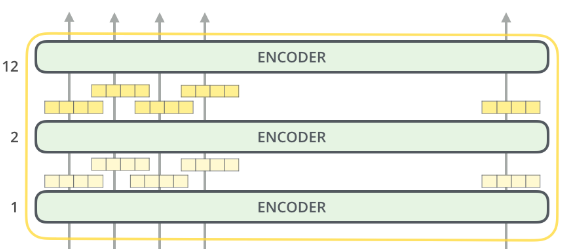
\includegraphics[width=\textwidth]{images/image212.png}
    \caption{Bert Embedding}
    \label{fig:bert_embeddings}
\end{center}
\end{figure}

\section{Learning to Rank} \label{sec:LTR}

Learning to Rank, \textit{LTR}, es una forma de aplicar técnicas de aprendizaje automático supervisado para resolver ciertas tareas en las cuales los objetivos son obtener un orden parcial. \textit{LTR} es bastamente utilizado en áreas tales como Information retrieval, PLN, Minería de Datos. La principal diferencia con las tareas de aprendizaje automático supervisado es que en estos el objetivo principal es obtener una predicción, ya sea regresión o clasificación, en cambio en las tareas de LTR el objetivo es obtener un ordenamiento óptimo de los ítems. En la Figura \ref{fig:learning_to_rank} podemos ver un ejemplo de un sistema de \textit{LTR} para el caso de Retrieval como puede ser un Motor de Búsqueda, en el ejemplo los $d_{i}$ serían los documentos o redirecciones a páginas disponibles, $q$ representa la búsqueda del usuario, y $d_{q,i}$ representa los primeros $n_{q}$ documentos. Nota: $d_{q} << d_{N}$.

Existen diferentes enfoques en los sistemas de \textit{LTR} tales como \textit{pointwise}, \textit{pairwise} y \textit{listwise}, la principal discrepancia entre estos radica en cuantos documentos consideramos en la función objetivo, loss function, durante el entrenamiento del modelo.

\begin{figure}
\begin{center}
    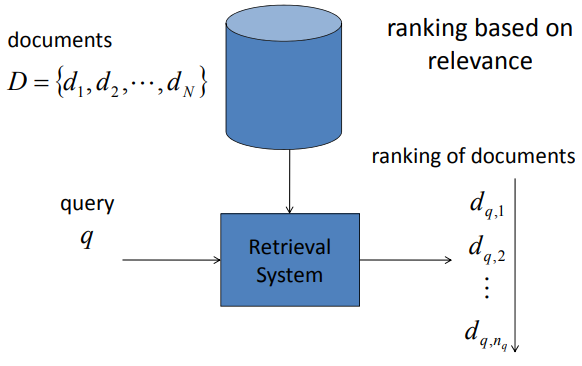
\includegraphics[width=\textwidth]{images/image207.png}
    \caption{Learning to Rank}
    \label{fig:learning_to_rank}
\end{center}
\end{figure}

\subsubsection{Pointwise}

Este enfoque mira un solo documento en la loss function, básicamente se entrena un clasificador/regresor y se trata de predecir cuán relevante es el documento, el ranking final es compuesto ordenando los $n_{q}$ documentos, cabe destacar que el score de cada documento es independiente de los otros documentos en el ordenamiento final.

\subsubsection{Pairwise} \label{sec:pairwise}

Este enfoque mira en la loss function documentos de a pares y trata de obtener el ranking óptimo. El objetivo es minimizar el número de inversiones en ordenamiento que el modelo predice, en la práctica este enfoque es mejor que el de pointwise ya que predecir el orden relativo modela mejor la realidad que predecir una relevancia. Unos ejemplos de estos algoritmos son \textit{RankNet}, \textit{LambdaRank} y \textit{LambdaMART} \cite{burges2010from}.

\subsubsection{Listwise} \label{sec:listwise}

Este enfoque mira directamente la lista entera de los documentos y trata de obtener el ordenamiento ideal. Unos ejemplos de estos algoritmos son \textit{SoftRank} \cite{taylor2008softrank}, \textit{ListMLE} \cite{inproceedings} y \textit{ListNet} \cite{cao2007learning}.
